\chapter{Question 3}
\section{Questions}
The power output, $P$, of a solar panel varies with the position of the sun. Let
$P(\theta) = 10\sin(\theta)$ watts, where $\theta$ is the angle between the
sun's rays and the panel, $0 \leq \theta \leq \pi$. On a typical summer day in
Ann Arbor, Michigan, the sun rises at 6am and sets at 8pm and the angle is
$\theta(t) = \pi\frac{t}{14}$ where $t$ is time in hours since 6am and
$0 \leq t \leq 14$.

\begin{enumerate}
  \item Write a formula for a function, $f(t)$, giving the power output of the
  solar panel (in watts), $t$ hours after 6am on a typical summer day in Ann
  Arbor.
  \item Graph the function $f(t)$ in the previous part for $0 \leq t \leq 14$.
  \item At what time is the power output greatest? What is the power output at
  this time?
  \item On a typical winter day in Ann Arbor, the sun rises at 8am and sets at
  5pm. Write a formula for a function, $g(t)$, giving the power output of the
  solar panel (in watts), $t$ hours after 8am on a typical winter day.
\end{enumerate}

\section{Solutions}
\begin{enumerate}
  \item We can write the function $P(\theta)$ in the following form
    \begin{align}
      f(t) &= 10\sin(k \cdot t) | 0 \leq t \leq 14 \\
      \intertext{where k is a value mapping the value of $t (0-14) \to \theta
      (0$ to $\pi)$}
      k &= \frac{\pi}{14}
      \intertext{such that at 6am}
      f(0) &= 10\sin(k \cdot 0) = 10\sin(0) = 0
      \intertext{and at 10pm (14 hours later)}
      f(14) &= 10\sin(k \cdot 14) = 10\sin(\pi) = 0
    \end{align}
    Thus the formula for the function we are looking for is
    \begin{center}
    \Huge{
      $f: (\mathbb{R}_{\geq 0} \to \mathbb{R}_{\leq 14}) \mapsto (0, 10)$\\
      $f(t) = 10\sin\left(\frac{t\cdot\pi}{14}\right)$
    }.
    \end{center}
  \item Graph of $f$ contained in figure \ref{fig:q3plot} on page
  \pageref{fig:q3plot}.
  \begin{figure}[!h]
    \centering
    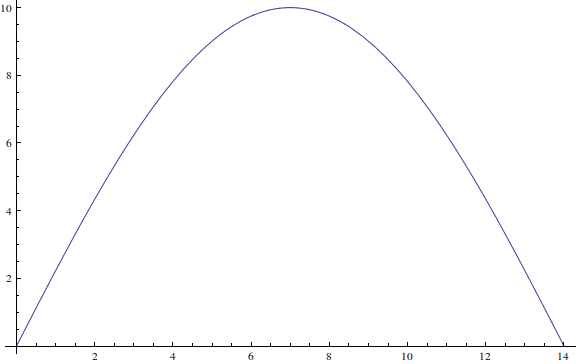
\includegraphics[width=\linewidth]{solutions/q3/q3plot.png}
  \caption{Plot of $f(t) = 10\sin\left(\frac{t\cdot\pi}{14}\right)$ from 0 to 14}
  \label{fig:q3plot}
  \end{figure}
  \item Power output will be at maximum when we are at a local maximum.
  Intuitively, this is 7 hours after 07:00, at 15:00 or 3pm. This can be
  confirmed with some differentiation of the function. To test for local maximum
  the following three conditions must be met:
  \begin{enumerate}
    \item at $t=7$ the derivative must be zero, and;
    \item at just before $t=7$ (say $t=6$) the derivative must be positive, and;
    \item at just after $t=7$ (say $t=8$) the derivative must be negative
  \end{enumerate}
  \begin{align}
    \intertext{test derivative of zero at $t=7$}
      f(t) &= 10\sin\left(\frac{t\cdot\pi}{14}\right) \nonumber \\
    \intertext{apply chain rule, let}
      u &= \frac{t \pi}{14} \nonumber
    \intertext{st}
      \frac{du}{dt} &= t \nonumber
    \intertext{and}
      \frac{d\sin(u)}{du} &= \cos(u) \\
    \intertext{st}
      \frac{d10\sin\left(\frac{t\cdot\pi}{14}\right)}{dt}
        &= \frac{d10\sin(u)}{du}\cdot \frac{d\frac{t\pi}{14}}{dt} \\
        &= \frac{d10\sin(u)}{du}\cdot \frac{\pi}{14} \\
        &= 10\frac{d\sin(u)}{du}\cdot \frac{\pi}{14} \\
        &= 10\cos(u)\cdot \frac{\pi}{14} \\
        &= \frac{5\pi}{7}\cos\left(\frac{t \pi}{14}\right) \label{eq:q2deriv}
    \intertext{evaluate at $t=7$}
      \frac{5\pi}{7}\cos\left(\frac{7 \pi}{14}\right) &= 0
    \intertext{evaluate at $t=6$}
      \frac{5\pi}{7}\cos\left(\frac{6 \pi}{14}\right) &\approx 0.499... \\
      & \quad \text{positive}
    \intertext{evaluate at $t=6$}
      \frac{5\pi}{7}\cos\left(\frac{8 \pi}{14}\right) &\approx -0.499... \\
      & \quad \text{negative}
  \end{align}
  $\therefore$ maximum at $t=7$ hours confirmed by increasing and decreasing
  gradients approaching $t=7$. The amount of power produced is 10 watts.
  \item A function, $g(t)$ representing the power output (P) of a panel can be
  constructed similarly to $f(t)$, except it will be compressed. Hours 0800 to
  1700 mean $k$ must map the range $0 \leq t \leq 9$ onto $0 \leq \theta \pi$

  \begin{align}
    g(t) &= 10\sin(k \cdot t) | 0 \leq t \leq 9 \\
    \intertext{where k is a value mapping the value of $t (0-9) \to \theta
    (0$ to $\pi)$}
    k &= \frac{\pi}{9}
    \intertext{such that at 8am}
    f(0) &= 10\sin(k \cdot 0) = 10\sin(0) = 0
    \intertext{and at 10pm (9 hours later)}
    f(9) &= 10\sin(k \cdot 9) = 10\sin(\pi) = 0
  \end{align}
  Thus the formula for the function we are looking for is
  \begin{center}
  \Huge{
    $g: (\mathbb{R}_{\geq 0} \to \mathbb{R}_{\leq 9}) \mapsto (0,10)$\\
    $g(t) = 10\sin\left(\frac{t\cdot\pi}{9}\right)$
  }.
  \end{center}
\end{enumerate}
